% arara: lualatex: { shell : yes }
% arara: lualatex: { shell : yes }
% arara: biber
% arara: lualatex: { shell : yes }
% arara: lualatex: { shell : yes }
% !TeX document-id = {d42c9162-1096-4f40-8a62-8cb41704ea7c}
% !TeX spellcheck = en_US
% !TeX TXS-program:compile = txs:///lualatex/[--shell-escape]
% !BIB program = biber

% !TEX root = slides.tex

\documentclass[
    %draft, % enable for quick rendering
    9pt,aspectratio=169,usepdftitle=false,
    %handout, % enable for uncover suppression
    hyperref={breaklinks},
    xcolor={svgnames}]{beamer}

% Load used-defined config
% !TEX root = slides.tex

\usepackage{expl3}
\usepackage{xparse}

%%%%%%%%%%%%
% Metadata %
%%%%%%%%%%%%

\ExplSyntaxOn

\tl_new:N   \l__configsupport_title_tl
\tl_new:N   \l__configsupport_author_tl
\tl_new:N   \l__configsupport_iso_date_tl
\tl_new:N   \l__configsupport_faculty_tl
\tl_new:N   \l__configsupport_chair_tl
\tl_new:N   \l__configsupport_workgroup_tl
\bool_new:N \l__configsupport_english_bool

\ProvideExpandableDocumentCommand{\settalktitle}{m}{
    \tl_set:Nn \l__configsupport_title_tl {#1}
}
\ProvideExpandableDocumentCommand{\talktitle}{}{\tl_use:N \l__configsupport_title_tl}

\ProvideExpandableDocumentCommand{\settalkauthor}{m}{
    \tl_set:Nn \l__configsupport_author_tl {#1}
}
\ProvideExpandableDocumentCommand{\addtalkauthor}{m}{
    \tl_if_empty:NF \l__configsupport_author_tl { \tl_put_right:Nn \l__configsupport_author_tl {,\ } }
    \tl_put_right:Nn \l__configsupport_author_tl {#1}
}
\ProvideExpandableDocumentCommand{\talkauthor}{}{\tl_use:N \l__configsupport_author_tl}

\ProvideExpandableDocumentCommand{\settalkisodate}{m}{
    \tl_set:Nn \l__configsupport_iso_date_tl {#1}
}
\ProvideExpandableDocumentCommand{\talkisodate}{}{\tl_use:N \l__configsupport_iso_date_tl}
\ProvideExpandableDocumentCommand{\talkdate}{}{\exp_args:Nf \DTMDate \talkisodate}

\ProvideExpandableDocumentCommand{\setfaculty}{m}{
    \tl_set:Nn \l__configsupport_faculty_tl {#1}
}
\ProvideExpandableDocumentCommand{\faculty}{}{\tl_use:N \l__configsupport_faculty_tl}

\ProvideExpandableDocumentCommand{\setchair}{m}{
    \tl_set:Nn \l__configsupport_chair_tl {#1}
}
\ProvideExpandableDocumentCommand{\chair}{}{\tl_use:N \l__configsupport_chair_tl}

\ProvideExpandableDocumentCommand{\setworkgroup}{m}{
    \tl_set:Nn \l__configsupport_workgroup_tl {#1}
}
\ProvideExpandableDocumentCommand{\workgroup}{}{\tl_use:N \l__configsupport_workgroup_tl}

\ProvideExpandableDocumentCommand{\germantalk}{}{
    \bool_set_false:N \l__configsupport_english_bool
}

\ProvideExpandableDocumentCommand{\englishtalk}{}{
    \bool_set_true:N \l__configsupport_english_bool
}

\ProvideExpandableDocumentCommand{\languagesetup}{}{
    \bool_if:NTF \l__configsupport_english_bool {
        \setdefaultlanguage[variant=usmax]{english}
        \setotherlanguage[variant=german, latesthyphen=true]{german}
    } {
        \setdefaultlanguage[variant=german, latesthyphen=true]{german}
        \setotherlanguage[variant=usmax]{english}
    }
}

\ExplSyntaxOff

%%%%%%%%%%%%%%%%%%%%%%
% Shorthand commands %
%%%%%%%%%%%%%%%%%%%%%%

\ProvideExpandableDocumentCommand{\aquaheader}{}{
    \setfaculty{Fakultät für Informatik}
    \setchair{Lehrstuhl 14 für Software Engineering}
    \setworkgroup{Arbeitsgruppe AQUA}
}
% !TEX root = slides.tex

%%%%%%%%%%%%%%%%%%
% Metadata setup %
%%%%%%%%%%%%%%%%%%

% Talk's title
\settalktitle{Meta Programming System: An Introduction}

% Author's name
\settalkauthor{Till Schallau}
% Multiple authors' names
% \addtalkauthor{John Doe}

% Talk date (ISO date format)
\settalkisodate{2020-09-28}

% Header metadata
\aquaheader

%%%%%%%%%%%%%%%%%%%%%%
% Language selection %
%%%%%%%%%%%%%%%%%%%%%%

%\germantalk
\englishtalk

%%%%%%%%%%%%
% Packages %
%%%%%%%%%%%%

% Should go first:

% Font control
\usepackage{fontspec}

% Math support
\usepackage{amsmath}
\usepackage{unicode-math}

% Font selection (needs to go before polyglossia)
\usepackage{libertinus}

% Language control
\usepackage{polyglossia}
\languagesetup

% Date formats
\usepackage[useregional]{datetime2}

% Algorithms
\usepackage[linesnumbered, vlined]{algorithm2e}

% Author and title reuse
\usepackage{authoraftertitle}

% Bibliography
\usepackage[style=alphabetic]{biblatex}

% Print-quality tables
\usepackage{booktabs}

% Watermarks for draft versions
%\usepackage{draftwatermark}
%\SetWatermarkAngle{57.5}
%\SetWatermarkLightness{.95}
%\SetWatermarkText{ENTWURF \(\alpha\).1}

% Image inclusion
\usepackage{graphicx}

% Enable microtypography support
\usepackage[final]{microtype}

% Listings with syntax highlighting; requires --shell-escape
\usepackage[newfloat]{minted}

% Fine spacing control for math
\usepackage{mleftright}

% PDF inclusion
\usepackage{pdfpages}

% Relative font sizes
\usepackage{relsize}

% URL's
\usepackage{url}

\usepackage[os=win]{menukeys}

% Drawings and Graphs
\usepackage{tikz}
\usetikzlibrary{babel}
\usetikzlibrary{calc}
\usetikzlibrary{external} % requires --shell-escape
\usetikzlibrary{positioning}
\tikzsetexternalprefix{tikz-externals}
% \tikzexternalize Render TikZ externally, fails for some references
\usepackage{pgfplots}
\pgfplotsset{compat=1.17}

% Needs to go last:

% Language-sensitive quotation marks
\usepackage{csquotes}

% Break URLs at / and -
\def\UrlBreaks{\do\/\do-}

%%%%%%%%%%%%%%%%%%%%
% Style and layout %
%%%%%%%%%%%%%%%%%%%%

% Load Theme
\usetheme{TUDo}
\titlegraphic{illustrations/Spektralringe}

% Neat + for et al
\renewcommand*{\labelalphaothers}{\raisebox{.3ex}{\relsize{-3}{\bfseries +}}}
\renewcommand*{\sortalphaothers}{+}

% Remove algorithm captions, see examples
\renewcommand{\AlCapSty}{}

% Use minted's line numbers for algorithm2e
\let\vrbstyle\theFancyVerbLine
\patchcmd{\vrbstyle}{\arabic{FancyVerbLine}}{}{}{}
\SetNlSty{vrbstyle}{}{}

% Pastel colored listings
\usemintedstyle{friendly}

% German strings
\addto\captionsgerman{%
    \renewcommand{\listlistingname}{Listingverzeichnis}%
}

%%%%%%%%%%%
% Content %
%%%%%%%%%%%

% Load external resources
\addbibresource{bibliography.bib}

% Internal metadata setup
\title{\talktitle}
\author{\talkauthor}
\date{\talkdate}

\institute{%
    \faculty

    \chair

    \workgroup%
}

\AtBeginSection[]{
    \begin{frame}<beamer>
        \frametitle{\contentsname}
        \tableofcontents[
            currentsection,
            currentsubsection,
            hideothersubsections,
            sectionstyle=show/shaded,
        ]
    \end{frame}
}

 \newcommand{\workshoplanguage}[1]{
\includegraphics[height=6px]{graphics/language.png} de.tudo.cs.ls14.aqua.mps.workshop.#1}

\newcommand{\workshoplanguagecreation}[0]{
\includegraphics[height=6px]{graphics/language.png} Language}
\newcommand{\workshopsolution}[1]{
\includegraphics[height=6px]{graphics/solution.png} de.tudo.cs.ls14.aqua.mps.workshop.#1}
\newcommand{\workshopmodel}[1]{
\includegraphics[height=6px]{graphics/model.png} #1}
\newcommand{\workshopnode}[1]{
\includegraphics[height=6px]{graphics/node.png} #1}
\newcommand{\workshopproject}[0]{
\includegraphics[height=6px]{graphics/project.png} mps-workshop}
\newcommand{\workshoprun}[0]{
\includegraphics[height=6px]{graphics/run.png} Run 'Node de.tudo.cs.ls14...'}
\newcommand{\workshopmoduleproperties}[0]{
\includegraphics[height=6px]{graphics/properties.png} Module Properties}
\newcommand{\workshopruntime}[0]{
\includegraphics[height=6px]{graphics/runtime.png} Runtime}
\newcommand{\workshopversion}[0]{\menu{
\includegraphics[height=6px]{graphics/version.png} Get from Version Control}}
\newcommand{\workshopinspector}[0]{
\includegraphics[height=6px]{graphics/inspector.png} Inspector}
\newcommand{\workshopintention}[0]{
\includegraphics[height=6px]{graphics/intention.png} Intention}


% Document content
\begin{document}
    \begin{frame}
        \setcounter{framenumber}{0}
        \titlepage
    \end{frame}

    \begin{frame}
        \frametitle{\contentsname}
        \tableofcontents[hideothersubsections]
    \end{frame}

    \section{Introduction}
    
    \begin{frame}{Meta Programming System}
    	The \textbf{Meta Programming System} (MPS) \footnote{\url{https://www.jetbrains.com/mps/}} is a language workbench to create \textbf{Domain Specific Languages} (DSL).\\
    	
    	MPS uses/provides:
    	\begin{itemize}
    		\item Code storage in an \textbf{Abstract Syntax Tree} (AST)
    		\item Projectional editing
    		\item Code generation
    		\item Language extension possibilities
    	\end{itemize}
    \end{frame}

	\begin{frame}{Abstract Syntax Tree}
		MPS is using an AST as its underlying model, therefore no specific parser is necessary.\\
		
		The language definition is based on AST-nodes, which build the abstract syntax tree.
		\begin{center}
			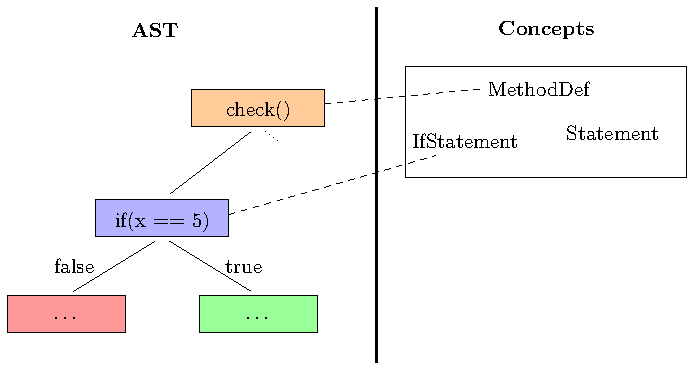
\includegraphics[height=0.7\textheight]{tikz/ast.pdf}
		\end{center}
	\end{frame}

	\begin{frame}{Projectional Editing}
		The \textbf{Projectional Editor} of MPS is a visual representation of the current AST. It is possible to have multiple editors with different presentation aspects.
		\begin{center}
			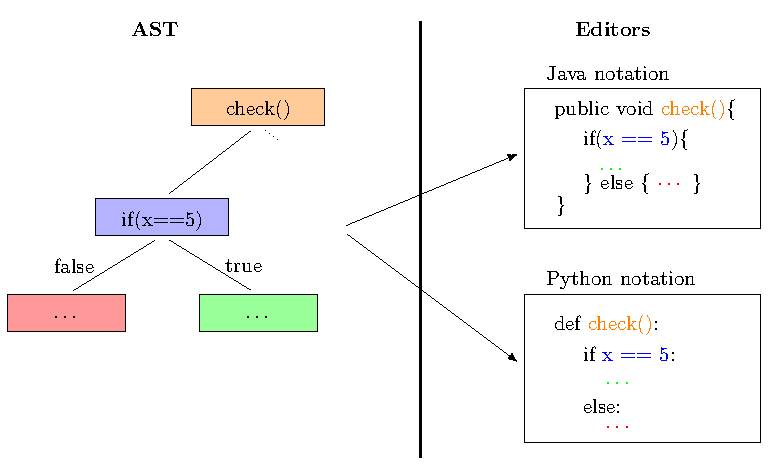
\includegraphics[height=0.7\textheight]{tikz/editors.pdf}
		\end{center}
	\end{frame}

	\begin{frame}{Hands-On}
		After this introduction into MPS, there is a repository with all necessary information under \url{https://github.com/tillschallau/mps-workshop}.\\
		
		In the now upcoming Hands-On part work on the \textbf{exercises 3.1 - 4.1}
	\end{frame}

	\begin{frame}{Model-Driven Engineering}
		\includegraphics[width=\textwidth]{tikz/mdsd_concept.pdf}
	\end{frame}

	\begin{frame}[noframenumbering]{Model-Driven Engineering}
		\includegraphics[width=\textwidth]{tikz/mdsd_concept_1.pdf}
	\end{frame}	
	
	\begin{frame}[noframenumbering]{Model-Driven Engineering}
		\includegraphics[width=\textwidth]{tikz/mdsd_concept_2.pdf}
	\end{frame}


	\section{Abstract Syntax}
	
	\begin{frame}{
\includegraphics[height=0.25cm]{graphics/concept.png}  Structure\footnote{\url{https://www.jetbrains.com/help/mps/structure.html}}}
		The structure of a language is defined as a \textbf{Concept} in MPS\\
		\begin{minipage}{0.52\textwidth}
			Concept:
			\begin{itemize}
				\item Inheritance
				\item Implementation of Interface
				\item Properties:
				\begin{itemize}
					\item Enumeration
					\item Primitive Datatype
					\item Constrained Datatype
				\end{itemize}
				\item Children:
				\begin{itemize}
					\item Any concept 
					\item Multiplicities ([1], [1..n], [0..n], [0..1])
				\end{itemize}
				\item References:
				\begin{itemize}
					\item Reference to another node
				\end{itemize}
			\end{itemize}
		\end{minipage}
		\begin{minipage}{0.4\textwidth}
			
\includegraphics[height=0.8\textheight]{illustrations/concept.png}
		\end{minipage}
	\end{frame}

	\begin{frame}
		\begin{center}
			\Huge \textbf{Hands-On}\\
			
			Exercise 4.2
		\end{center}
	\end{frame}

	\section{Concrete Syntax}
	
	\begin{frame}{Model-Driven Engineering}
		\includegraphics[width=\textwidth]{tikz/mdsd_concept_3.pdf}
	\end{frame}

	\begin{frame}[noframenumbering]{Model-Driven Engineering}
		\includegraphics[width=\textwidth]{tikz/mdsd_concept_4.pdf}
	\end{frame}

	\begin{frame}{\includegraphics[height=0.25cm]{graphics/editor.png}  Editor\footnote{\url{https://www.jetbrains.com/help/mps/editor.html}}}
		\begin{minipage}{0.52\textwidth}
			Types of Cell Models:
			\begin{itemize}
				\item \textbf{Constant cell}: \texttt{<constant>}
				\item \textbf{Property cell}: \texttt{\{property\}}
				\item \textbf{Child cell}: \texttt{\%child\%}
				\item \textbf{Referent cell}: \texttt{(\%reference\%->\{name\})}
				\item \textbf{Child list cell}: \texttt{(>\%child\%/empty cell: <default><)}
				\item \textbf{Model access}: \texttt{*model access*}
				\item \textbf{Collection cell}: \texttt{[- -]} (indent layout) or \\
				\textcolor{white}{Collection cell: n} \texttt{[> <]} (horizontal) or \\
				\textcolor{white}{Collection cell: n} \texttt{[/ /]} (vertical) 
			\end{itemize}
		\end{minipage}
		\begin{minipage}{0.4\textwidth}
			\includegraphics[height=0.8\textheight]{illustrations/editor.png}
		\end{minipage}
	\end{frame}

	\begin{frame}{\includegraphics[height=0.25cm]{graphics/transformation.png} Transformations\footnote{\url{https://www.jetbrains.com/help/mps/transformation-menu-language.html}}}
	\begin{minipage}{0.52\textwidth}
		Transformations let you edit the AST by replacing \\
		and moving AST nodes\\
		
		\textbf{Example:}\\
		\texttt{(x and y)} type \menu{or} should yield \\
		\texttt{((x and y) or \_)}\\
		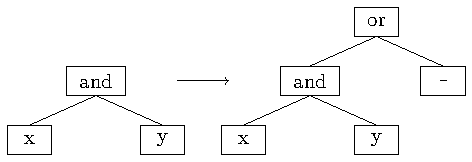
\includegraphics[height=0.4\textheight]{tikz/transformation.pdf}
	\end{minipage}
	\begin{minipage}{0.4\textwidth}
		\includegraphics[height=0.75\textheight]{illustrations/transformation.png}
	\end{minipage}
	\end{frame}

	\begin{frame}{
\includegraphics[height=0.25cm]{graphics/intentions.png} Intentions\footnote{\url{https://www.jetbrains.com/help/mps/mps-intentions.html}}}
		\begin{minipage}{0.52\textwidth}
			Intentions:
			\begin{itemize}
				\item Provide \menu{\workshopintention} menu by pressing \menu{Alt}+\menu{\return}
				\item Execute predefined actions
				\item Can be used to correct errors (\textbf{error intention})
			\end{itemize}
			Variants:
			\begin{itemize}
				\item Intention
				\item Universal Intention
				\item Surround With Intention
				\item Parameterized Intention
			\end{itemize}
		\end{minipage}
		\begin{minipage}{0.4\textwidth}
			
\includegraphics[height=0.8\textheight]{illustrations/intention.png}
		\end{minipage}
	\end{frame}

	\begin{frame}
		\begin{center}
			\Huge \textbf{Hands-On}\\
			
			Exercises 4.3 - 4.5
		\end{center}
	\end{frame}

	\section{Static Semantics}
	
	\begin{frame}{Model-Driven Engineering}
		\includegraphics[width=\textwidth]{tikz/mdsd_concept_5.pdf}
	\end{frame}
	
	\begin{frame}[noframenumbering]{Model-Driven Engineering}
		\includegraphics[width=\textwidth]{tikz/mdsd_concept_6.pdf}
	\end{frame}
		
	\begin{frame}{
\includegraphics[height=0.25cm]{graphics/checkingrules.png} Checking Rules\footnote{\url{https://www.jetbrains.com/help/mps/typesystem.html}}}
		\begin{minipage}{0.52\textwidth}
			Checks:
			\begin{itemize}
				\item Inspect the model for known error patterns
				\item Static code analysis
				\item Reports found errors/warnings/infos
				\item Can provide quick fixes for errors/warnings
			\end{itemize}
		\end{minipage}
		\begin{minipage}{0.4\textwidth}
			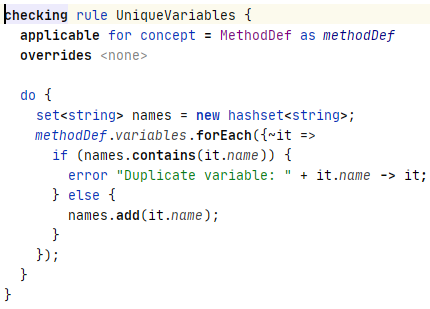
\includegraphics[height=0.8\textheight]{illustrations/check.png}
		\end{minipage}
	\end{frame}
	
	\begin{frame}{
\includegraphics[height=0.25cm]{graphics/quickfix.png} Quick Fixes\footnote{\url{https://www.jetbrains.com/help/mps/typesystem.html}}}
		\begin{minipage}{0.52\textwidth}
			Quick Fixes can be attached to the \texttt{error}, \texttt{warning}\\
			or \texttt{info} call in a checking rule via the \\
			\menu{\workshopinspector{}} menu
		\end{minipage}
		\begin{minipage}{0.4\textwidth}
			
\includegraphics[height=0.8\textheight]{illustrations/quickfix.png}
		\end{minipage}
	\end{frame}

	\begin{frame}
		\begin{center}
			\Huge \textbf{Hands-On}\\
			
			Exercise 4.6
		\end{center}
	\end{frame}

	\section{Semantics}
	
	\begin{frame}{Model-Driven Engineering}
		\includegraphics[width=\textwidth]{tikz/mdsd_concept_7.pdf}
	\end{frame}
	
	\begin{frame}[noframenumbering]{Model-Driven Engineering}
		\includegraphics[width=\textwidth]{tikz/mdsd_concept_8.pdf}
	\end{frame}
	
	\begin{frame}{Language Generation}
		In MPS there are two possible ways of generating (here: transforming) code.\\
		
		\begin{minipage}{0.4\textwidth}
			\textbf{Model-To-Model Transformation}
		\end{minipage} 
		\begin{minipage}{0.09\textwidth}
			\Large
			\textcolor{white}{$\Rightarrow$}
		\end{minipage}
		\begin{minipage}{0.4\textwidth}
			\textbf{Model-To-Text Transformation}
		\end{minipage}
	
		\vspace*{0.5cm}
		\pause
		
		\begin{minipage}{0.4\textwidth}
			\begin{itemize}
				\item Translate models into other models
				\item Predefined models exist:
				\begin{itemize}
					\item Base Language (Java)
					\item mbeddr (C and C extensions) \footnotemark[8]
					\item MPS CSharp (C\#) \footnotemark[9]
				\end{itemize}
				\item Does not flush text into file
				\item Each predefined model has an associated Model-To-Text Transformation
			\end{itemize}
		\end{minipage} 
		\footnotetext[8]{\url{http://mbeddr.com/}}
		\footnotetext[9]{\url{https://github.com/vaclav/MPS_CSharp}}
		\pause
		\begin{minipage}{0.09\textwidth}
			\Large
			$\Rightarrow$
		\end{minipage}
		\begin{minipage}{0.4\textwidth}
			\begin{itemize}
				\item Convert a model into text
				\item Give the output some reasonable layout
				\item Lets you define a file ending (e.g. \texttt{.java})
				\item Flush text into a file
			\end{itemize}
		\end{minipage}
	\end{frame}

	\begin{frame}{Model-To-Model Transformation \footnote[10]{\url{https://www.jetbrains.com/help/mps/generator-language.html}}}
		\begin{minipage}{0.52\textwidth}
			Each generator consists of \textbf{\workshopconfiguration s} that combines all templates\\
			
			Some Generator Rules:\\
			\begin{itemize}
				\item \textbf{Root Mapping Rule:} Generates a root node in the output model
				\item \textbf{Reduction Rule:} Transforms a node based on a template
				\item \textbf{Mapping Label:} Helper for name consistency throughout generation
			\end{itemize}
		\end{minipage}
		\begin{minipage}{0.4\textwidth}
			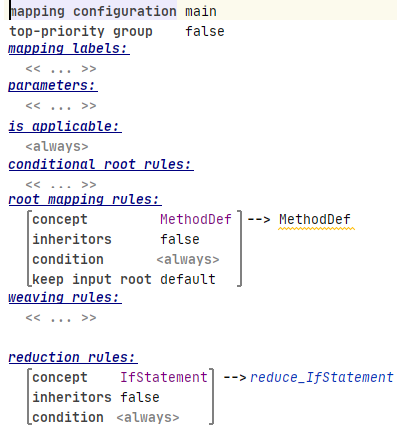
\includegraphics[height=0.85\textheight]{illustrations/mapping.png}
		\end{minipage}
	\end{frame}

	\begin{frame}{\workshoptemplate s \footnote[11]{\url{https://www.jetbrains.com/help/mps/generator-language.html}}}
		\begin{minipage}{0.52\textwidth}			
			Template Macros used in a \textbf{Template Fragment <TF TF>}:\\
			\begin{itemize}
				\item \textbf{Property \$[]:} Computes value of a property
				\item \textbf{Reference ->\$[]:} Computes referent node
				\item \textbf{\$IF\$[]:} Conditional generation of template code
				\item \textbf{\$LOOP\$[]:} Applies template to set of nodes
				\item \textbf{\$CALL\$[]:} Calls another template with parameters
				\item \textbf{\$COPY\_SRC\$[]:} Copies node
				\item \textbf{\$LABEL\$[]:} Registers generated name into generation context
			\end{itemize}
		\end{minipage}
		\begin{minipage}{0.4\textwidth}
			
\includegraphics[height=0.5\textheight]{illustrations/template.png}
			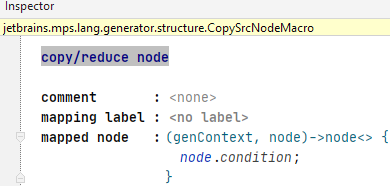
\includegraphics[height=0.38\textheight]{illustrations/template_inspector.png}
		\end{minipage}
	\end{frame}

	\begin{frame}{\workshoptemplate\ Combination 1/4}
	\begin{minipage}{0.52\textwidth}
		Lets wrap the \texttt{MethodDef} concept into a newly created concept  \texttt{ClassDef}
	\end{minipage}
	\begin{minipage}{0.4\textwidth}
		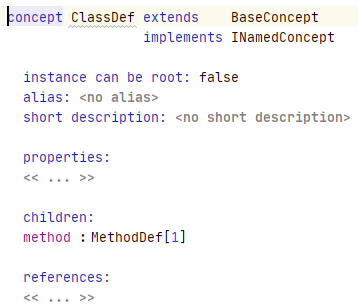
\includegraphics[height=0.8\textheight]{illustrations/classDef.png}
	\end{minipage}
	\end{frame}

	\begin{frame}{\workshoptemplate\ Combination 2/4}
	\begin{minipage}{0.52\textwidth}
		The \texttt{ClassDef} generator template contains a statically generated method \texttt{print()}\\
		
		The \texttt{ClassDef} generator template contains the generated output of the \texttt{MethodDef} concept
	\end{minipage}
	\begin{minipage}{0.4\textwidth}
		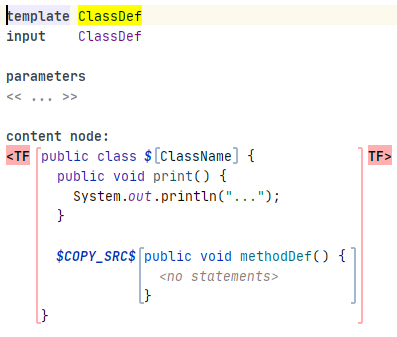
\includegraphics[height=0.8\textheight]{illustrations/classDefGen.png}
	\end{minipage}
	\end{frame}

	\begin{frame}{\workshoptemplate\ Combination 3/4}
	\begin{minipage}{0.52\textwidth}
		To generate the method, generate its children: \\
		\begin{itemize}
			\item \texttt{Variables} (e.g. \texttt{\$COPY\_SRCL\$[String s = "";]})
			\item \texttt{Statements} (e.g. \texttt{\$COPY\_SRCL\$[s = "";]})
		\end{itemize}
	
		\textcolor{white}{m}\\
		
		If we now want to call the \texttt{print}-method of the \texttt{ClassDef}-concept, the current template has to be enhanced, as the method is currently not available in our context.
	\end{minipage}
	\begin{minipage}{0.4\textwidth}
		\includegraphics[height=0.8\textheight]{illustrations/methodDefGen.png}
	\end{minipage}
	\end{frame}

	\begin{frame}{\workshoptemplate\ Combination 4/4}
	\begin{minipage}{0.52\textwidth}
		To use the \texttt{print}-method, simulate the surrounding environment necessary for the generation (e.g. the surrounding class with its \texttt{print()}-method)\\
		
		Mark the code that should be generated with the \texttt{Template Fragment} macro
	\end{minipage}
	\begin{minipage}{0.4\textwidth}
		\includegraphics[height=0.8\textheight]{illustrations/methodDefGen2.png}
	\end{minipage}
	\end{frame}

	\begin{frame}
		\begin{center}
			\Huge \textbf{Hands-On}\\
			
			Exercise 4.7
		\end{center}
	\end{frame}

	\begin{frame}{\workshoptextgen\ \footnote{\url{https://www.jetbrains.com/help/mps/textgen.html}}}
	\begin{minipage}{0.52\textwidth}
		The TextGen language operations:\\
		\begin{itemize}
			\item \textbf{append:} append text of the following kind:
			\begin{itemize}
				\item \textbf{\{string value\}:} constant text
				\item \textbf{\textbackslash n:} line break
				\item \textbf{\$list\{node.list\}:} list without separator
				\item \textbf{\$list\{node.list with ,\}:} list with separator ``,''
				\item \textbf{\$\{node.child\}}
			\end{itemize}
			\item \textbf{with indent \{ code \}:} increase indentation level for \texttt{code}
			\item \textbf{indent buffer:} apply indentation for current line
			\item \textbf{increase depth:} increase indentation level
			\item \textbf{decrease depth:} decrease indentation level
		\end{itemize}
	\end{minipage}
	\begin{minipage}{0.4\textwidth}
		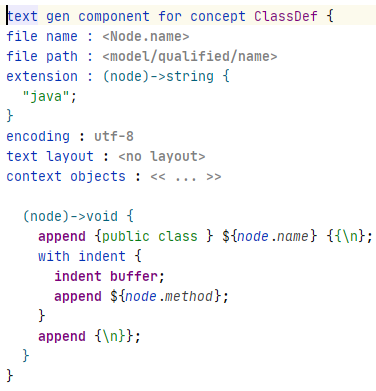
\includegraphics[height=0.9\textheight]{illustrations/textgen.png}
	\end{minipage}
	\end{frame}

	\begin{frame}
		\begin{center}
			\Huge \textbf{End of the workshop}\\
			
			Have a nice evening
		\end{center}
	\end{frame}	
\end{document}